 \documentclass{articleUL} 
 \usepackage[pdftex]{graphicx}
\usepackage{graphics}
\usepackage{amsmath}
\usepackage{color}
\usepackage{tikz}
\usepackage{titlesec}
\usepackage{hyperref}
\usepackage{pdfpages}
\titleclass{\subsubsubsection}{straight}[\subsection]

\newcounter{subsubsubsection}[subsubsection]
\renewcommand\thesubsubsubsection{\thesubsubsection.\arabic{subsubsubsection}}
\renewcommand\theparagraph{\thesubsubsubsection.\arabic{paragraph}} % optional; useful if paragraphs are to be numbered

\titleformat{\subsubsubsection}
  {\normalfont\normalsize\bfseries}{\thesubsubsubsection}{1em}{}
\titlespacing*{\subsubsubsection}
{0pt}{3.25ex plus 1ex minus .2ex}{1.5ex plus .2ex}

\makeatletter
\renewcommand\paragraph{\@startsection{paragraph}{5}{\z@}%
  {3.25ex \@plus1ex \@minus.2ex}%
  {-1em}%
  {\normalfont\normalsize\bfseries}}
\renewcommand\subparagraph{\@startsection{subparagraph}{6}{\parindent}%
  {3.25ex \@plus1ex \@minus .2ex}%
  {-1em}%
  {\normalfont\normalsize\bfseries}}
\def\toclevel@subsubsubsection{4}
\def\toclevel@paragraph{5}
\def\toclevel@paragraph{6}
\def\l@subsubsubsection{\@dottedtocline{4}{7em}{4em}}
\def\l@paragraph{\@dottedtocline{5}{10em}{5em}}
\def\l@subparagraph{\@dottedtocline{6}{14em}{6em}}
\makeatother

\setcounter{secnumdepth}{4}
\setcounter{tocdepth}{4}
\usetikzlibrary{positioning}
\usepackage{adjustbox}
\usepackage{float}
 \title{GMC-7004, Sujet Spécial (génie mécanique). Système d'exploitation de robot, ROS, environnement de simulation.} 
 %% You can add up to 7 differents authors
 \author{Philippe Lebel
 \affiliation{Université Laval, philippe.lebel.4@ulaval.ca}}
 \begin{document}
 \selectlanguage{french}	% Change to "francais" if needed
 \maketitle
 \begin{abstract}
L'objectif de ce sujet spécial est de rendre compte des connaissances acquises pour l'utilisation de différents outils de développement dans le domaine de la robotique. Les différentes problématiques abordées dans ce rapport sont: la communication ordinateur-robot sans l'entremise d'un noeud de calcul, l’installation et utilisation de la plateforme ROS et la mise sur pied d'un environnement de simulation robotique en utilisant des outils tels que Gazebo, V-rep et URSIM. L'objectif étant de démontrer l'acquisition de connaissances mais aussi de permettre à d'autres d'utiliser cette synthèse, le présent rapport tente d'exemplifier et a une approche pratique sur l'utilisation des outils mentionnés.
\end{abstract}
 \documentclass[root.tex]{subfiles}
\begin{document}


\section{Introduction}
Dans une démarche expérimentale, il est souvent requis d'implémenter les algorithmes développés, dans un environnement tel que Matlab, sur des systèmes robotiques déjà existants. 
La solution couramment utilisée est d'employer un nœud de calcul QNX sur lequel RTLAB est installé. 
Ceci requiert un processus d'adaptation autant au niveau de l'utilisation du logiciel qu'au niveau de l'adaptation du code Matlab, python c++ déjà développé. 
Bien souvent, le processus peut s'échelonner sur plusieurs semaines. 
Ceci motive alors la recherche d'alternatives permettant l'utilisation directe du code sur un système robotique. 
L'objectif étant de permettre l'utilisation de différents langage de programmation pour minimiser le temps d'adaptation. 
Une solution permettant l'utilisation du code Matlab, python, c++ et autre est alors mise sur pied.

\section{Mise en contexte}

Les solutions présentées dans ce rapport répondent toutes au besoin d'utiliser le code directement sur un montage robotique. 
Cependant, elle présentent toutes différents avantage et inconvénient. 
Comme processus de validation, le solutions ont été testées en répondant à la même problématique: l'utilisation d'un bras Jaco de Kinova directement par l'entremise de la connexion usb.


\section{Définition des objectifs}

Différents critères doivent être rencontrés pour qu'une solution soit acceptable et remplace le système déjà en place.

\begin{enumerate}
\item Permettre la communication bidirectionnelle.
\item Être compatible avec plusieurs systèmes robotiques.
\item Permettre une communication avec un délais de moins de 10 ms. (100 Hz)
\item Permettre une grande flexibilité dans le type de commandes qu'un utilisateur peut envoyer. (commandes articulaires, cartésiennes, force, etc.)
\end{enumerate}

\section{Solution de contrôle du bras Jaco développée sous Windows}

Sachant que Windows est le système d'exploitation majoritairement utilisé au sein du laboratoire de robotique de l'université Laval, le besoin de développer une solution compatible Windows a été identifié. 
La stratégie employée est représenté dans la Figure \ref{fig:diag}.
\begin{figure}
 \begin{center}
  \begin{tabular}{c}
    \includegraphics[trim=0cm 0cm 0cm 0cm, scale=0.17]{"diag_fonc3".pdf}
  \end{tabular}
 \end{center}
\caption{General structure of the algorithm.}
 \label{fig:diag}
\end{figure}
Du point de vue global, la structure du système se résume en une chaine de communication UDP entre différents programmes et le robot. 
Cependant, dans le cas de l'implémentation avec le robot Jaco, une API, \textit{Applications Programming Interface}, gère l'interface entre les actionneurs et les requêtes communiquées au robot via la connection USB.
Dans le cas du Jaco, cette API permet l'utilisation de différentes fonctions rédigées en c++.
Ceci cause problème lorsqu'un développeur tente d'utiliser un programme écrit en Matlab ou en python pour commander les articulations du robots.
La solution à cet inconvénient est d'initier une instance Matlab via un un script c++.
Cette instance Matlab pourra ensuite exécuter des commandes que le script c++ lui envoi, tel que l’exécution de fonctions Matlab.
Par la suite, il suffit d'utiliser directement l'API de kinova pour envoyer des commandes.

\subsection{Exemple d'implémentation}

Différents composants doivent être mis en place pour réaliser l'implémentation.
Le présent exemple permet de configurer un projet visual studio pour contrôler un bras Jaco en communiquant avec Matlab.
\subsubsection{Visual Studio}
Il est possible de télécharger \href{https://www.visualstudio.com/thank-you-downloading-visual-studio/?sku=Community&rel=15}{VisualStudio} sur le site web des développeurs.

\subsubsection{Création d'un projet}
Un projet VisualStudio peut être créé en cliquant sur \textit{file/new/project} dans la fenêtre de visual studio.
Ensuite, sélectionner \textit{Visual c++} dans le menu gauche de la nouvelle fenêtre et cliquez sur \textit{Empty Project}.
Dans le bas de la fenêtre, il est possible de nommer le projet et sélectionner un répertoire.
Le répertoire choisi sera référé comme étant le \textit{workspace} ou \textit{project direcotry} dans la pluspart des tutoriels en anglais.
Tout ficher placé dans ce répertoire fera partie du projet et pourra être référé dans les scripts.

\subsubsection{Définition du fichier principal du projet}
Pour être en mesure d'écrire le script, un fichier source doit être créé.
Pour créer ce ficher, il faut cliquer droit sur l'item \textit{Source Files} dans l'arbre du projet situé à la droite de la fenêtre Visual Studio.
Ensuite, il faut sélectionner \textit{add/new item} et cliquer sur \textit{c++ File}.
Il est ensuite possible de nommer le fichier dans le bas de la fenêtre.

\subsubsection{Utilisation d'un joystick}
Pour être en mesure d'envoyer des commandes avec un joystick, la librairie \href{https://www.libsdl.org/release/SDL2-2.0.7.zip
}{SDL2} doit être téléchargée.
Bien sûr, si le projet ne requiert pas de contrôleur joystick, cette étape n'est pas nécessaire.
Après avoir décompressé le dossier téléchargé, lire le fichier VisualC.html pour les instructions sur la démarche à suivre pour utiliser la libraire (en particulier la partie parlant de l'utilisation avec Visual Studio).
Les détails de l'utilisation pratique de cette librairie seront couverts dans une section subséquente.

\subsubsection{Lien avec Matlab}

La description de cette partie se fera en deux temps.
Dans un premier temps, une explication des différentes composantes devant être mises en places pour monter l'environnement de développement sera présentée.
Ensuite, l'installation des pilotes pour l'envoie de commandes au bras Jaco est expliquée.
\paragraph{Environnement de travail} Les différentes librairies, exécutables et les entêtes (\textit{headers})  nécessaires à l'utilisation de Matlab via un script c++ sont disponible dans le répertoire retourné lorsque l'on envoie les commandes suivantes dans la console Matlab:
\begin{enumerate}
\item fullfile(matlabroot,'bin','win64').
\item fullfile(matlabroot,'extern','include'),
\item fullfile(matlabroot,'extern','lib'),
\end{enumerate}

Pour les utiliser dans un projet Visual Studio, il est nécessaire de suivre les étapes suivantes:
\begin{itemize}
\item Il est tout d'abord très important de s'assurer que l'option x64 est sélectionnée dans le menu déroulant dans le haut et au centre de la fenêtre principale de Visual Studio.
\item Aller dans \textit{Project\textbackslash'nom-de-votre-projet' Properties...} dans le haut de la fenêtre principale de Visual Studio.
\item Naviguer dans l'onglet Debugging de la fenêtre venant de s'ouvrir.
\item Écrire \textit{PATH=} suivi du résultat obtenu lors de l'envoie de la commande 1 dans le console Matlab, en omettant les guillemets,(devrait ressembler à \newline \textit{C:\textbackslash Program Files\textbackslash MATLAB\textbackslash R2017b\textbackslash bin\textbackslash win64}) dans le section \textit{Environnement}.
Écrire Directement à la suite de la dernière entrée: \textit{;\%PATH\%}
\item Naviguer dans l'onglet VC++ Directories de la même fenêtre.
\item \textbf{Pour les prochaines étapes}: Si un item était déjà présent dans cette ligne, il faut simplement séparer les entrées avec un ";".
\item Insérer le résultat obtenu lors de l'envoie de la commande 2 dans le console Matlab, en omettant les guillemets, dans le section \textit{Include Directories}.
\item Insérer le résultat obtenu lors de l'envoie de la commande 3 dans le console Matlab, en omettant les guillemets, dans le section \textit{Library Directories}.
\item Naviguer dans l'onglet \textit{Linker} et le sous-onglet \textit{Input} de la même fenêtre.
\item Entrer au début d'\textit{Additional Dependencies} l'entrée suivante: \textit{libmx.lib;libeng.lib;libmex.lib;libmat.lib;}
\end{itemize}

Pour tester l'environnement de travail, un script c++ est inclu avec les version récentes de Matlab. 
Il est accessible en entrant la commande:
\begin{itemize}
\item $ edit([ matlabroot $\textbackslash$ extern$\textbackslash$ examples$\textbackslash$ eng\_mat$\textbackslash$ engdemo.cpp' ]);$
\end{itemize}

Il faut seulement copier-coller l'entièreté du script dans le fichier source (.cpp) du projet Visual Studio. Le clic sur le bouton \textit{Local Windows Debugger} lancera la compilation et devrait faire apparaitre un invité de commande. 
La première compilation est normalement beaucoup plus longue que les compilations subséquente.

\paragraph{Installation de Kinova SDK}
Pour être en mesure d'envoyer des commandes au robot jaco, il est nécessaire d'installer les pilotes fournis sur le site web de \href{https://drive.google.com/open?id=0B790iVm0vRTlRFNFRldIb2Jmbkk}{Kinova}.
Suivant l'installation de Kinova SDK, des directives doivent être suivies pour que le robot soit bien reconnu par le système d'exploitation.
Ces directives sont disponible dans le répertoire d'installation de \textit{KinovaSDK\textbackslash Guides\textbackslash Kinova SDK-User Guide} (souvent situé dans \textit{Program Files x86}).
Pour tester l'envoi de commandes au robot et valider l'installation, une interface graphique est disponible dans \textit{KinovaSDK\textbackslash GUI}.
Des exemples de scripts c++ sont aussi disponibles dans le répertoire \textit{KinovaSDK\textbackslash Examples}.


À la suite du test, il est maintenant possible de combiner les informations des deux tutoriels pour faire fonctionner des scripts matlab, transférer des données de l'environnement de travail matlab vers le \textit{stack} du programme c++ et vice versa.

\subsection{Conclusion}

Dans cette section, un survol de l'implémentation de l'environnement de développement permettant le contrôle du bras Jaco sous Windows avec l'option d'utiliser des scripts Matlab a été présentée.
Bien que seulement le bras Jaco a été mentionné, il est toutefois possible d'utiliser les API \textit{c++} d'autres systèmes robotiques tels que les bras de Universal Robot. 
Cependant, une autre option pour contrôler le bras UR5 sous windows est disponible.
Cette dernière est présentée dans la section suivante.

\end{document}
\newpage



















 
 
 \begin{thebibliography}{}
 \bibitem{key1} First Reference...
 \end{thebibliography}
 \newpage
 \appendix
\section{\\Manuel de programmation URscript} \label{app:URscript_manual}

% the \\ insures the section title is centered below the phrase: Appendix A

\includepdf[pages=-, offset=75 -75]{scriptmanual_en_3_1.pdf}

\section{\\Fonctions de l'API VRep} \label{app:VRep_manual}

% the \\ insures the section title is centered below the phrase: Appendix A
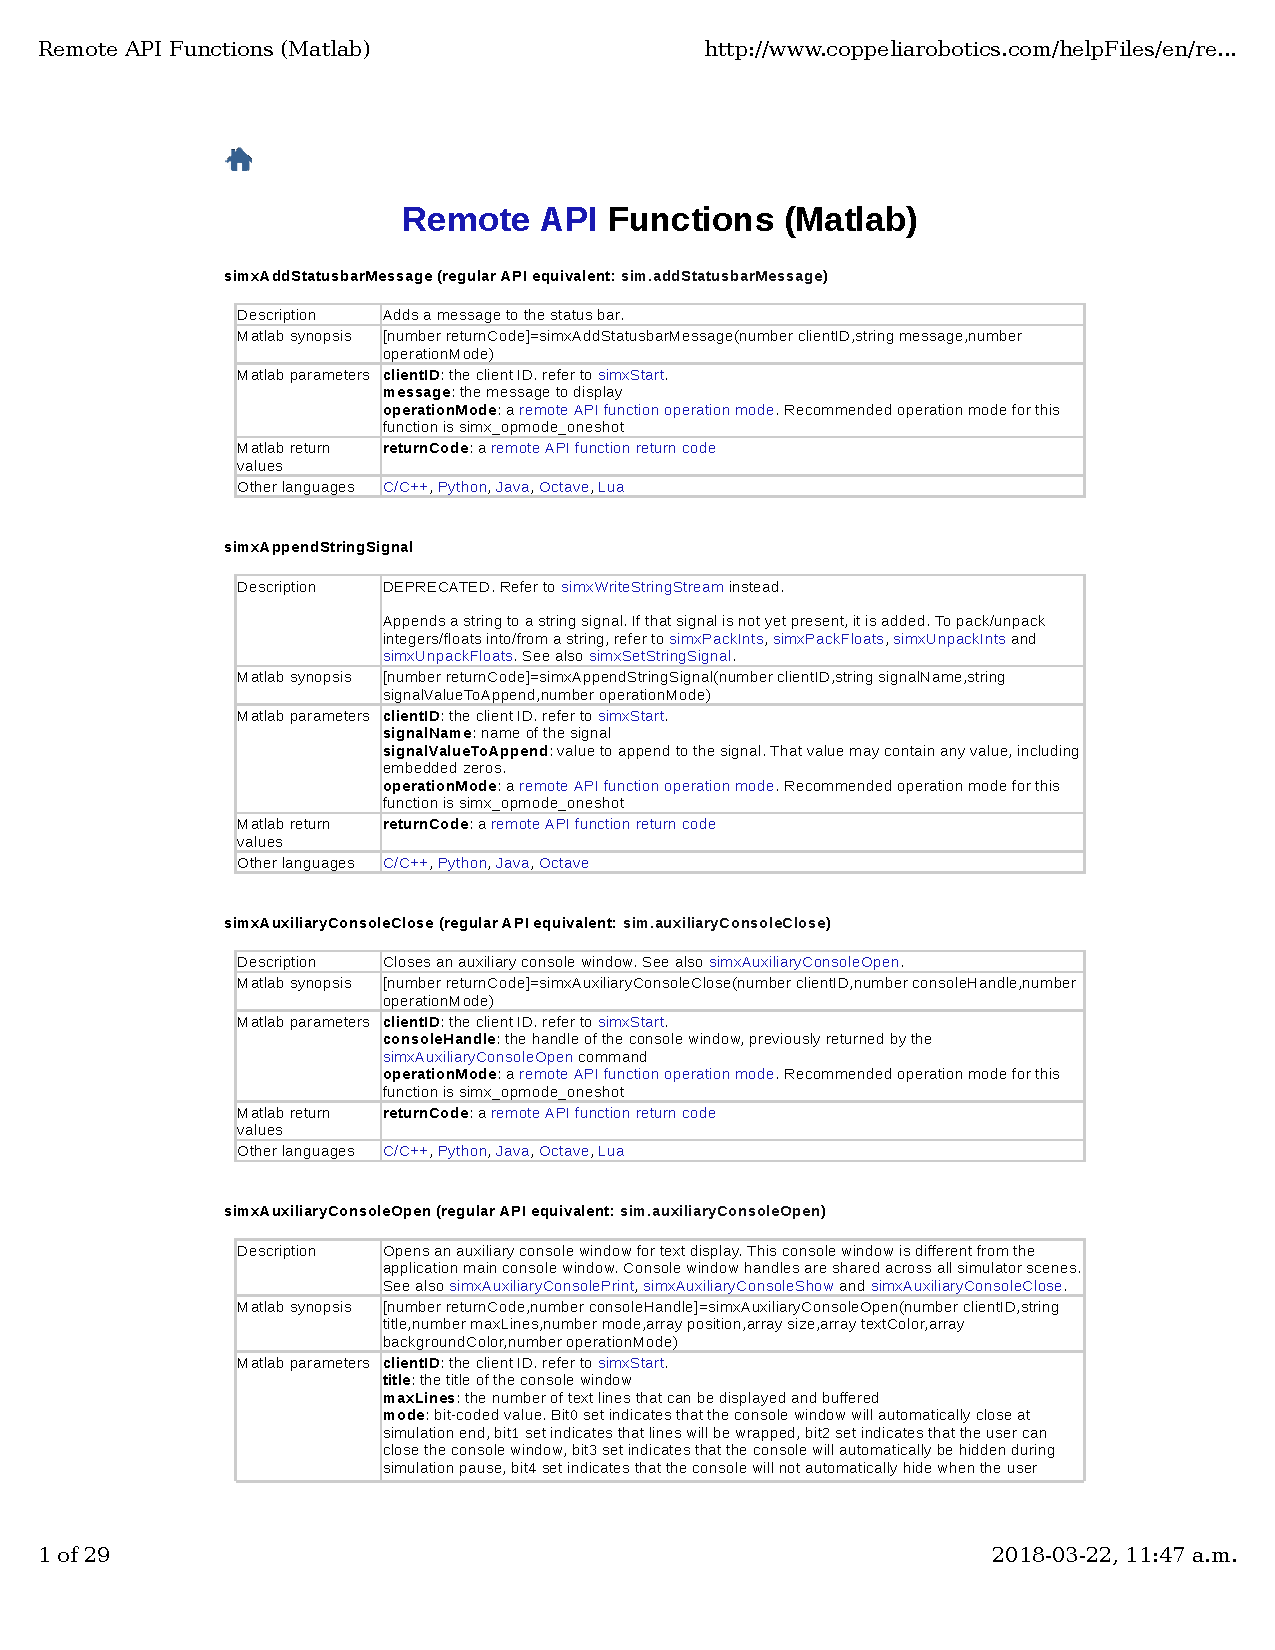
\includepdf[pages=-, offset=75 -75]{VRep_manual.pdf}
 \end{document} 